\begin{center}
\Large \textbf{Chapter 5: The Generative Lexicon, \\ a Case Study} \\[1ex]
\end{center} 
\setcounter{section}{0}
Thus far, we have approached the linguistic issue, i.e. the problem of interpreting the atoms of lexical decomposition, at a very high theoretical level. An abstract mathematical system has been offered to facilitate the interpretation, complete with a theorem that establishes a way in which semantic atoms and concepts can be regarded as identical. Conversely, we have approached the cognitive science issue from a mostly empirical perspective; the mathematical tools introduced here are offered as a model of empirical results about conceptual hierarchy and typicality. Little has been done to \emph{apply} the mathematics to theories of lexical decomposition, in order to gain understanding of linguistic phenomena, and even less has been done to make use of the formalism as a set of theoretical tools to answer questions for cognitive scientists. In this chapter, we will fill in some remaining gaps and demonstrate, via case study, how to \emph{use} inheritance networks to answer real questions. James Pustejovsky's \emph{Generative Lexicon} \cite{pustejovsky_generative_1998} is the case we will study.

In Section \ref{GL}, Chapter 2, I have already explained the basics of the Generative Lexicon. In the present chapter, I will expand on the earlier explanation by looking more closely at two of Pustejovsky's generative rules. Where linguistics is concerned, Pustejovsky provides a formal model of how word senses are generated in cases of systematic polysemy, but the model is just that---purely formal. Equipped with the theorem of Chapter 4, we will be able to look ``under the hood,'' so to speak, in order to gain a better understanding of the cognitive mechanism that enables us to understand novel word senses, at least in the cases where word senses are generated according to Pustejovsky's rules.

Cognitive scientists often use linguistic stimuli as a way to study concepts. In some of the experiments outlined in Chapter 3, subjects where primed with sentences and asked to respond. But words (and therefore sentences) are only an intermediary for what cognitive scientists are really interested in, which is concepts. There is very good reason to believe that the same word can stand for different concepts in different contexts (more on this below), and therefore cognitive scientists are faced with the problem of identifying cases where two instances of a word do stand for the same concept, as well as cases where they do not.

For example, suppose a cognitive scientist studying the influence of hierarchy on inference primes subjects with the following sentences:\footnote{In reality, it would probably be more likely to see cognitive scientists asking subjects to rate their willingness to infer (iii$^\prime$) ``Josh is reading a book.'' from (ii$^\prime$) ``Josh is reading a novel.'' I have constructed this artificial example because it is consistent with the problems that will be raised in this chapter. Although somewhat artificial, it is not entirely implausible, since cognitive scientists may want to compare the effects of hierarchy in inferences of different logical form.}
\begin{enumerate}[(i)]
\item Josh is about to begin reading.
\item Josh is holding a novel.
\end{enumerate}
The scientist might then ask test subjects to rate their willingness to infer:
\begin{enumerate}[(i)]
\setcounter{enumi}{2}
\item Josh is about to begin a book.
\end{enumerate}
The idea is that we might test whether subjects are willing to accept this inference on the grounds that {\bf novel} is subordinate to {\bf book} in the hierarchy. But this only tests the influence of hierarchy if the senses of ``novel'' and ``book'' are senses that correspond to use of the concepts {\bf novel} and {\bf book}. We shall soon see, by means of a slightly modified example, that there is good reason to think that the sense of ``book'' in (iii) does not correspond to the concept {\bf book}.

The theorem of Chapter 4 is an isomorphism, i.e.\ a relation-preserving bijection between two domains. These domains, called isomorphs, are regarded as mathematically indistinguishable, and therefore a main value of an isomorphism is that things learned in one domain can be extended into the other. We can answer the linguistic question by looking at how functional roles of concepts vary under generative rules, and we can answer (part of) the cognitive science question by making use of the formalism offered in decompositional lexical semantics. These questions will be answered simultaneously, not due to careful selection of examples, necessarily, but rather because it is a consequence of the theorem that they are in fact the same question approached from different angles.

\section{``Josh began the novel.''}

Let's begin with an example.\footnote{I have modified things slightly in this section from what was including in our toy example above. This was done because the semantics dealth with here will be more intuitive and natural to deal with than what would be required to deal directly with the sentences used above. The basic ideas, however, are the same, and it should not be too difficult for the reader to see how what is said here relates to what has been said above.} Consider the sentence ``Josh began the novel.'' The kinds of things we begin are events; beginning is always beginning \emph{to do} something. But the object of ``began,'' in this sentence, is ``the novel,'' which is not an event. Nevertheless, any native speaker of English will find this to be a perfectly comprehensible sentence. We are, therefore, faced with something of a puzzle: our understanding of the concepts represented by the words in this sentence implies that the sentence should be conceptually incoherent, but the sentence is obviously coherent.

We take the sentence to mean is that Josh is beginning to do something to/with/etc.\ the novel. There is an implicit event that is being begun, which is not syntactically realized, and ``the novel'' is something on which or with which the implicit event is being performed. For example, two very natural ways of understanding the sentence are ``Josh began reading the novel'' and ``Josh began writing the novel.'' The conceptual question is whether the concept {\bf novel} is, in fact, an event concept (i.e., a representation of a category of actions, rather than a category of objects)---contrary to intuitions---or whether ``the novel'' stands for a more complex concept of {\bf reading the novel} or {\bf writing the novel} in this sentence. The linguistic question is how the semantics of ``the novel'' can allow it to be coherently used as an argument for ``began.'' James Pustejovsky has answered the linguistic question for us, by defining a generative rule that makes use of inheritance networks to resolve the type error. By trading on the mathematical indistinguishability of the aspects of semantic content that are represented in inheritance networks and conceptual hierarchy, we can make use of his formal answer to the linguistic question in answering the conceptual question.

\subsection{True Complement Coercion}

Recall the following (partial) typed feature structures for ``novel'' and ``begin'' from Chapter 2:
\par\vspace{5mm}
$$\left[
\begin{array}{l l}
\textbf{novel} & \\
\mathcal{A} = & \left[ \begin{array}{l}
				\text{ARG}_1=\textbf{x:book} \\
				\end{array}\right] \\
\mathcal{Q} = & \left[ \begin{array}{l}
				\text{CONST}=\textbf{narrative(x)} \\
				\text{FORMAL}=\textbf{x} \\
				\text{TELIC}=\textbf{read(y,x)} \\
				\text{AGENT}=\textbf{write(y,x)}
				\end{array}\right] \\
\end{array}
\right]$$
\par\vspace{5mm}
$$\left[
\begin{array}{l l}
\textbf{begin} & \\
\mathcal{A} = & \left[ \begin{array}{l}
	\text{ARG}_1=\textbf{y:animate\_obj} \\
	\text{ARG}_2=\textbf{z:event}_1 \\
	\end{array}\right] \\
\mathcal{E} = & \left[ \begin{array}{l}
	\text{E}_1=\textbf{transition} \\
	\mathellipsis \\
	\end{array}\right] \\
\mathcal{Q} = &  \left[ \begin{array}{l}
	\text{FORMAL}=\textbf{P(event}_1\textbf{,y)} \\
	\text{AGENT} = \textbf{begin\_act(event}_1\textbf{y,z)} \\
	\end{array}\right] \\
\end{array}
\right]$$
\par\vspace{5mm}
The types given in the typed feature structures are supplied by the following inheritance network (ignore the colors for the time being; we will make use of them shortly):
\begin{center}
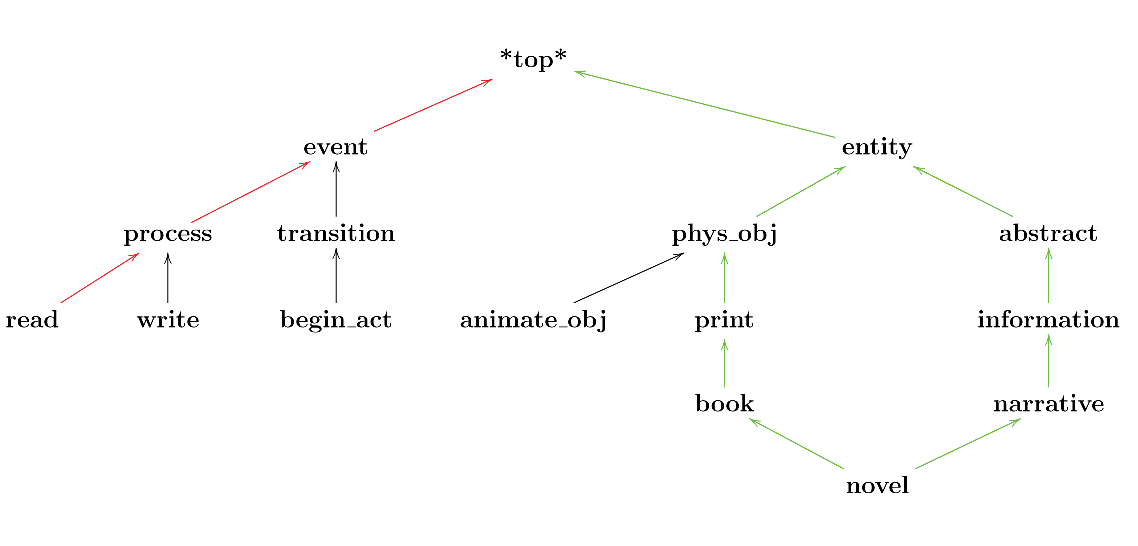
\includegraphics[width=4.75in]{InheritanceNetwork}
\vspace{3mm}
Figure 1
\end{center}

We can read the argument expectations for ``begin'' directly off of the typed feature structure. In particular, we see that ``begin'' expects a direct object of type {\bf event}; this type assignment is a representation of our intuition that events are the kinds of things that can be begun. Since ``novel'' is not a verb, as has been explained, its argument structure specifies the default behavior of ``novel'' when it is used as an argument; it behaves as an argument of type {\bf book}. But, as can be read off of the inheritance network, {\bf book} does not inherit from {\bf event}, so the sentence ``Josh began the novel'' entails a violation of the type expectations for arguments of ``begin.''

According to Pustejovsky, we resolve the type error by applying a generative rule that searches the qualia structure of ``begin'' for some type that inherits from {\bf event}.\footnote{Pustejovsky does offer a formal definition of this rule. His formalization is quite opaque, however, and I think unpacking it will take us needlessly afield from the main point, since the general idea behind the rule can be understood to the degree required here without the formalization.} In fact, we find that the qualia structure of ``novel'' includes two qualia, i.e.\ TELIC and AGENT, whose assigned types inherit from {\bf event}; we read off of the graph that both {\bf read} and {\bf write} inherit from {\bf event}. Coercing ``novel'' to behave as an argument of type {\bf read} or {\bf write} leads us to understand ``Josh began the novel'' as ``Josh began \emph{to read} the novel'' or ``Josh began \emph{to write} the novel,'' respectively.\footnote{In fact, Pustejovsky faces something of a problem here: there are other possible readings of ``Josh began the novel.'' In some unusual cases, we might think of readings such as ``Josh began to eat the novel'' or ``Josh began to skim the novel,'' and it isn't clear how Pustejovsky's qualia can accommodate the seemingly innumerable readings we might conceive of.}

In fact, type coercion isn't \emph{merely} shifting from one type to another. Pustejovsky states, informally, that ``true type coercion \emph{involves} the strict shifting of one type to another specified type $\mathellipsis$ but embeds the existing type into the resulting type by the proper coercion operation'' \cite[p.\ 115]{pustejovsky_generative_1998}. Formally and computationally, how this is done can be read off of the typed feature structure for ``novel''. In the argument structure of ``novel,'' we see that the default behavior of ``novel'' is specified as {\bf x:book}. But this reads ``{\bf x} of type {\bf book},'' where {\bf x} is a variable that takes the value ``novel'' in the sentence ``Josh began the novel.''\footnote{We actually have multiple variables at play in ``Josh began the novel.'' ``Josh'' is a value taken by the variable {\bf y} in the typed feature structure for ``begin,'' which is designated to be of type {\bf animate\_obj}. Since Josh is an animate object, no type error, and therefore no coercion, occurs.}  If we observe that each of the qualia is a function of {\bf x}, we see that the coercion is not to {\bf read}, but to {\bf read(x)}, which is understood as {\bf read(a novel)} (ignoring the definite article).

Pustejovsky's type coercion is closely related to Barsalou's \emph{ad hoc} categories \cite{barsalou_adhoc_1983}. Barsalou makes the point that some categories are well-established in memory, and therefore we have familiar, well-established concepts to represent those categories. However, in practice we make use of novel categories all the time. For example, Barsalou points out that we might be faced with a situation in which we need to make use of the category ``things to take from one's home during a fire.'' Surely, we have no well-worn concept to represent this category. (Much pity on anyone who does!) Because we lack such a concept, there seem to be no identifiable features among items in the category (such as children, pets, laptop computers, etc.) that serve to bind the category together by family resemblance. Nevertheless, we are able to form and make use of the necessary concepts ``on-the-fly,'' when the need arises.\footnote{Baralou's theory of ad hoc categories is, incidentally, predicated largely off of Rosch's work. I have no particular opinion on how and whether this observation relates to the project of this thesis; I bring it up merely as a point of interest.}

Likewise, we have a word ``novel'' with a well-worn sense that corresponds to the concept {\bf novel}. Pustejovsky's type coercion is a model of the mechanism by which we create an \emph{ad hoc} word sense ``on-the-fly'' when the need arises. The default argument behavior of ``novel'' is given by the type assignment of the feature ARG$_1$. Since novel behaves as an argument of type {\bf x:book}, we take this to mean that the default (or ``well-worn'') sense of ``novel'' corresponds to some concept that inherits from {\bf book}, i.e.\ the concept {\bf novel}. When the argument behavior of ``novel'' is coerced to a new type, we are then faced with the question of whether the new type (read: concept) is identical with the original one.

We might recall from Section \ref{sec2}, Chapter 4, that identity betweeen functional roles is a necessary condition for identity between concepts. The functional role $i(\textbf{novel})$ is highlighted in green in the above graph. A consistent definition $D_\textbf{read}$ is highlight in red. We can read directly off of the graph that $D_\textbf{read}\notin i(\textbf{novel})$. But, by the definition of $i(\textbf{read})$, we know that $D_\textbf{read}\in i(\textbf{read})$. Therefore, $i(\textbf{read})\neq i(\textbf{novel})$, and therefore the concept being represented by ``novel'' in ``Josh begain the novel'' cannot be the concept {\bf novel}. We have answered the question of whether the concepts corresponding to each sense of ``novel'' are identical.

\section{Another example: ``Mary drives a Honda.''}

Consider the sentences:
\begin{enumerate}[(i)]
\item Mary drives a Honda.
\item Mary bought stock in Honda.
\end{enumerate}

We only have one word ``Honda,'' which refers to both a category of cars and a car-manufacturing company. We might wonder, however, whether these are both different parts or aspects of the same concept {\bf Honda}. After all, the two domains of reference are clearly related to one another, and in fact the very reason we use the word ``Honda'' to refer to the category of cars is because they are made by Honda, the car manufacturer. Does ``Honda'' correspond to a single concept, which is a representation of a category that includes both the cars and the manufacturer? Or do these two uses of ``Honda'' correspond to distinct concepts?

Some typed feature structures:
\par\vspace{5mm}
$$\left[
\begin{array}{l l}
\textbf{drive} & \\
\mathcal{A} = & \left[ \begin{array}{l}
	\text{ARG}_1=\textbf{x}:\textbf{human} \\
	\text{ARG}_2=\textbf{y}:\textbf{vehicle} \\
	\end{array}\right] \\
\mathcal{E} = & \left[ \begin{array}{l}
	\text{E}_1=\textbf{e}_1:\textbf{process} \\
	\text{E}_2=\textbf{e}_2:\textbf{process} \\
	\text{RESTR}=<\circ_\propto
	\end{array}\right] \\
\mathcal{Q} = &  \left[ \begin{array}{l}
	\text{FORMAL}=\textbf{move}(\textbf{e}_2,\textbf{y}) \\
	\text{AGENT} = \textbf{drive\_act}(\textbf{e}_1,\textbf{x},\textbf{y}) \\
	\end{array}\right] \\
\end{array}
\right]$$
\par\vspace{5mm}
$$\left[
\begin{array}{l l}
\textbf{buy stock} & \\
\mathcal{A} = & \left[ \begin{array}{l}
	\text{ARG}_1=\textbf{x}:\textbf{human}
	\text{ARG}_2=\textbf{y}:\textbf{coporation}
	\end{array}\right] \\
\mathcal{E} = & \left[ \begin{array}{l}
	\text{E}_1=\textbf{e}_1:\textbf{transition} \\
	\end{array}\right] \\
\mathcal{Q} = &  \left[ \begin{array}{l}
	\text{FORMAL}=\textbf{transfer\_ownership}(\textbf{e},\textbf{x},\textbf{stock\_share},\textbf{y}) \\
	\text{TELIC}=\textbf{gain}(\textbf{e},\textbf{x},\textbf{profit}) \\
	\text{AGENT} = \textbf{trade}(\textbf{e},\textbf{x},\textbf{y}) \\
	\end{array}\right] \\
\end{array}
\right]$$
\par\vspace{5mm}

I have omitted feature structures for the senses of ``Honda'' since it isn't clear or important to understand whether and/or how one sense of ``Honda'' is generated from the other by type coercion. Creating a feature structure for ``Honda'' would require ironing out these issues and identifying an appropriate generative rule, which would be messy (to say the least) and would take us too far afield from the present task. Everything we need to know can be seen from the following inhertance hierarchy, which provides the types we need:
\begin{center}
\includegraphics[width=4.75in]{InheritanceNetwork2}
\vspace{3mm}
Figure 2
\end{center}

We know from the argument structures of ``drive'' and ``buy stock'' that the sense of ``Honda'' in (i) must display argument behavior of type {\bf vehicle}, while the sense of ``Honda'' in (ii) must display argument behavior of type {\bf corporation}. Again, we can read directly off of the graph that $D_\textbf{Honda-Co}\notin i(\textbf{Honda})$, and therefore $\textbf{Honda-Co}$ and $\textbf{Honda}$ cannot be the same concept.

\section{Some final remarks}

It is important to realize that the diagnostic demonstrated here is only a diagnostic for non-identity between concepts. Since the framework of inheritance networks and consistent definitions does not provide a sufficient condition for identity of concepts, we cannot establish that two concepts $\alpha$ and $\beta$ \emph{are} identical unless we are able to check that \emph{every possible} $D_\alpha\in i(\beta)$. This would only be possible, in principle, if the number of possible $D_\alpha$'s is finite, and there is no reason to suppose that this is true. (I suspect that it is not.)

Also, the Theorem and the conceptual interpretation of semantic atoms have no consequence for the formalism in GL, i.e.\ the generative rules, the features, and the structure of lexical entries are unaffected by the interpretation. (Or for the formalism in any theory of lexical decomposition.) They do have consequences for the meta-theories of lexical decomposition, however, in that they give a deeper account of \emph{why} such theories have the features they do, by interpreting the atoms as concepts. In the case of GL, we are now equipped to understand type coercion as remapping the relation between concepts and words (in cases where the diagnostic justifies  this understanding). Also, since cognitive scientists have already developed a robust set of empirical tools for studying conceptual hierarchy, we can now make use of those tools to determine which inhertance networks are admissable in theories of lexical decomposition.

For theories of lexical decomposition that dictate specific inheritance relations, we can turn toward cognitive science to determine whether these relations are empirically justified. For theories of lexical decomposition like GL, which leave wide open the question of what our inheritance networks should look like, we now have an empirical means for discovering the right inheritance networks to use. The details of how this can be done are outside the scope of this thesis. In fact, obtaining the same results I did when applying the diagnostic above relies crucially on having set up the inheritance hierarchies in the way that I have. Getting the right inheritance network is a matter of getting the right hierarchy relations, and so the diagnostic always ``faces the tribunal of sense experience,'' to borrow some of Quine's words, in that empirical discoveries always have the final say about how to set up the inheritance network. Note: Since the point of these questions is that distinct types can represent the same concept, provided they have the same functional roles, including {\bf Honda} and {\bf Honda-Co} as separate atoms does not ``stack the deck'' in favor of regarding them as distinct concepts. This does not mean that, in practice, we must engage in an empirical study of hierarchy at the outset for every inheritance network we want to define. For the most part, our intuitions about what is a plausible hierarchy should suffice---it would seem very strange indeed to place {\bf animal} subordinate to {\bf human}---but empirical data can serve as an arbiter, when challenges against a particular network are raised.

\section{Summary}

We can make use of the isomorphism to study semantic atoms by looking at concepts and vice versa. Taking GL as a case study allows us to see how the functional role $i$ can provide us with diagnostics to determine whether two distinct uses of a word represent the same concept. In making use of diagnostics to establish that the functional roles of the concepts being represented by words are not identical, we can infer that the concepts are not identical. However, the framework of inheritance networks affords us with no known diagnostic to establish that two concepts \emph{are} identical. Such a diagnostic would require possession of a sufficient condition for identity of concepts, but the tools defined here can only provide us with a necessary condition for identity of concepts.

\clearpage
